\documentclass[10pt,utf8]{beamer}

\mode<presentation> {
  \usetheme{Madrid}
  \setbeamercovered{transparent}
}

\usepackage{palatino}
\usepackage{graphicx}
\usepackage{array}
\usepackage{color}
\usepackage{subfigure}
\usepackage{colortbl}
\usepackage{amsmath}
\usepackage{hyperref}
\usepackage{listings}
\usepackage{pythonhighlight} % dnf install texlive-pythonhighlight

\setbeamertemplate{caption}{\raggedright\insertcaption\par} %turn off caption prefix ("Figure")

\definecolor{delim}{RGB}{20,105,176}
\definecolor{numb}{RGB}{106, 109, 32}
\definecolor{string}{rgb}{0.64,0.08,0.08}


\title{Debezium Asynchronous Engine}
\author{Vojtěch Juránek}
\institute[Red Hat]{Red Hat}
\date{May 21st 2024, Debezium F2F meeting, Brno}

\newenvironment{mylisting}
{\begin{list}{}{\setlength{\leftmargin}{1em}}\item\scriptsize\bfseries}
{\end{list}}

\newenvironment{mytinylisting}
{\begin{list}{}{\setlength{\leftmargin}{1em}}\item\tiny\bfseries}
{\end{list}}


\begin{document}

\begin{frame}
    \titlepage
\end{frame}

\begin{frame}
    \frametitle{Debezium embedded engine}
    \begin{figure}
        \centering
        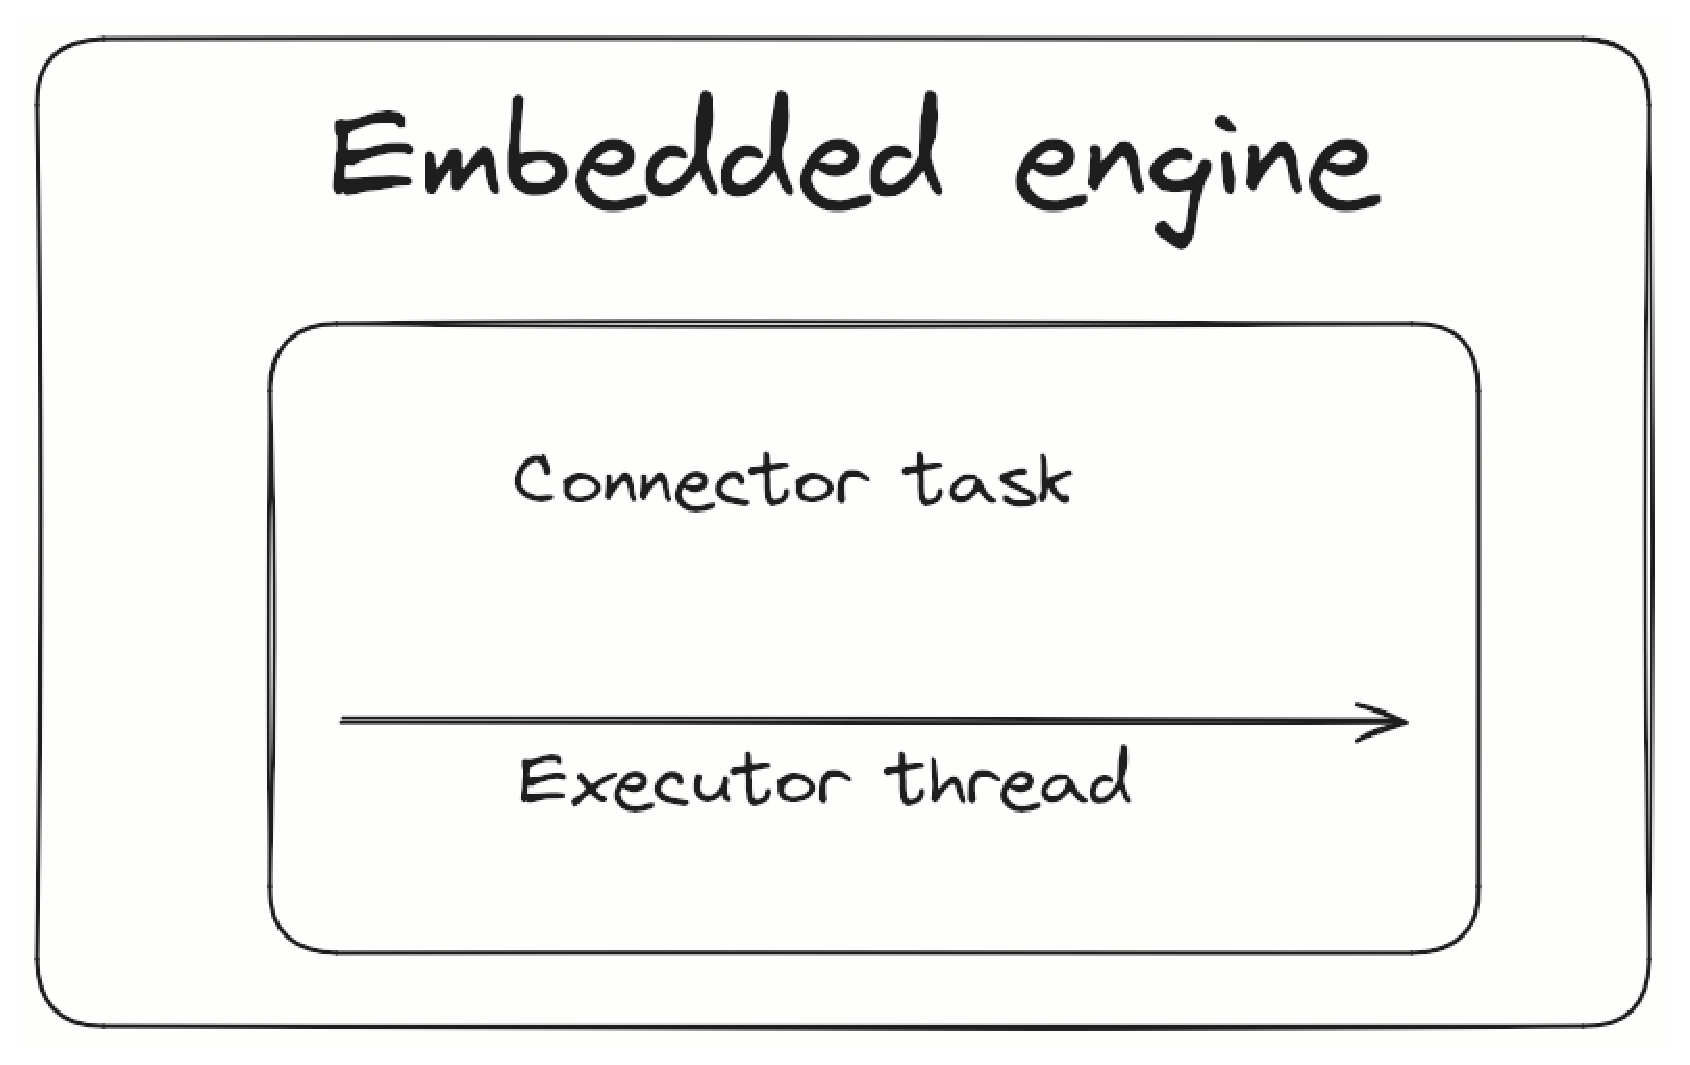
\includegraphics[height=6cm]{./img/embedded_engine.eps}
    \end{figure}
\end{frame}

\begin{frame}
    \frametitle{Debezium asynchronous engine}
    \begin{figure}
        \centering
        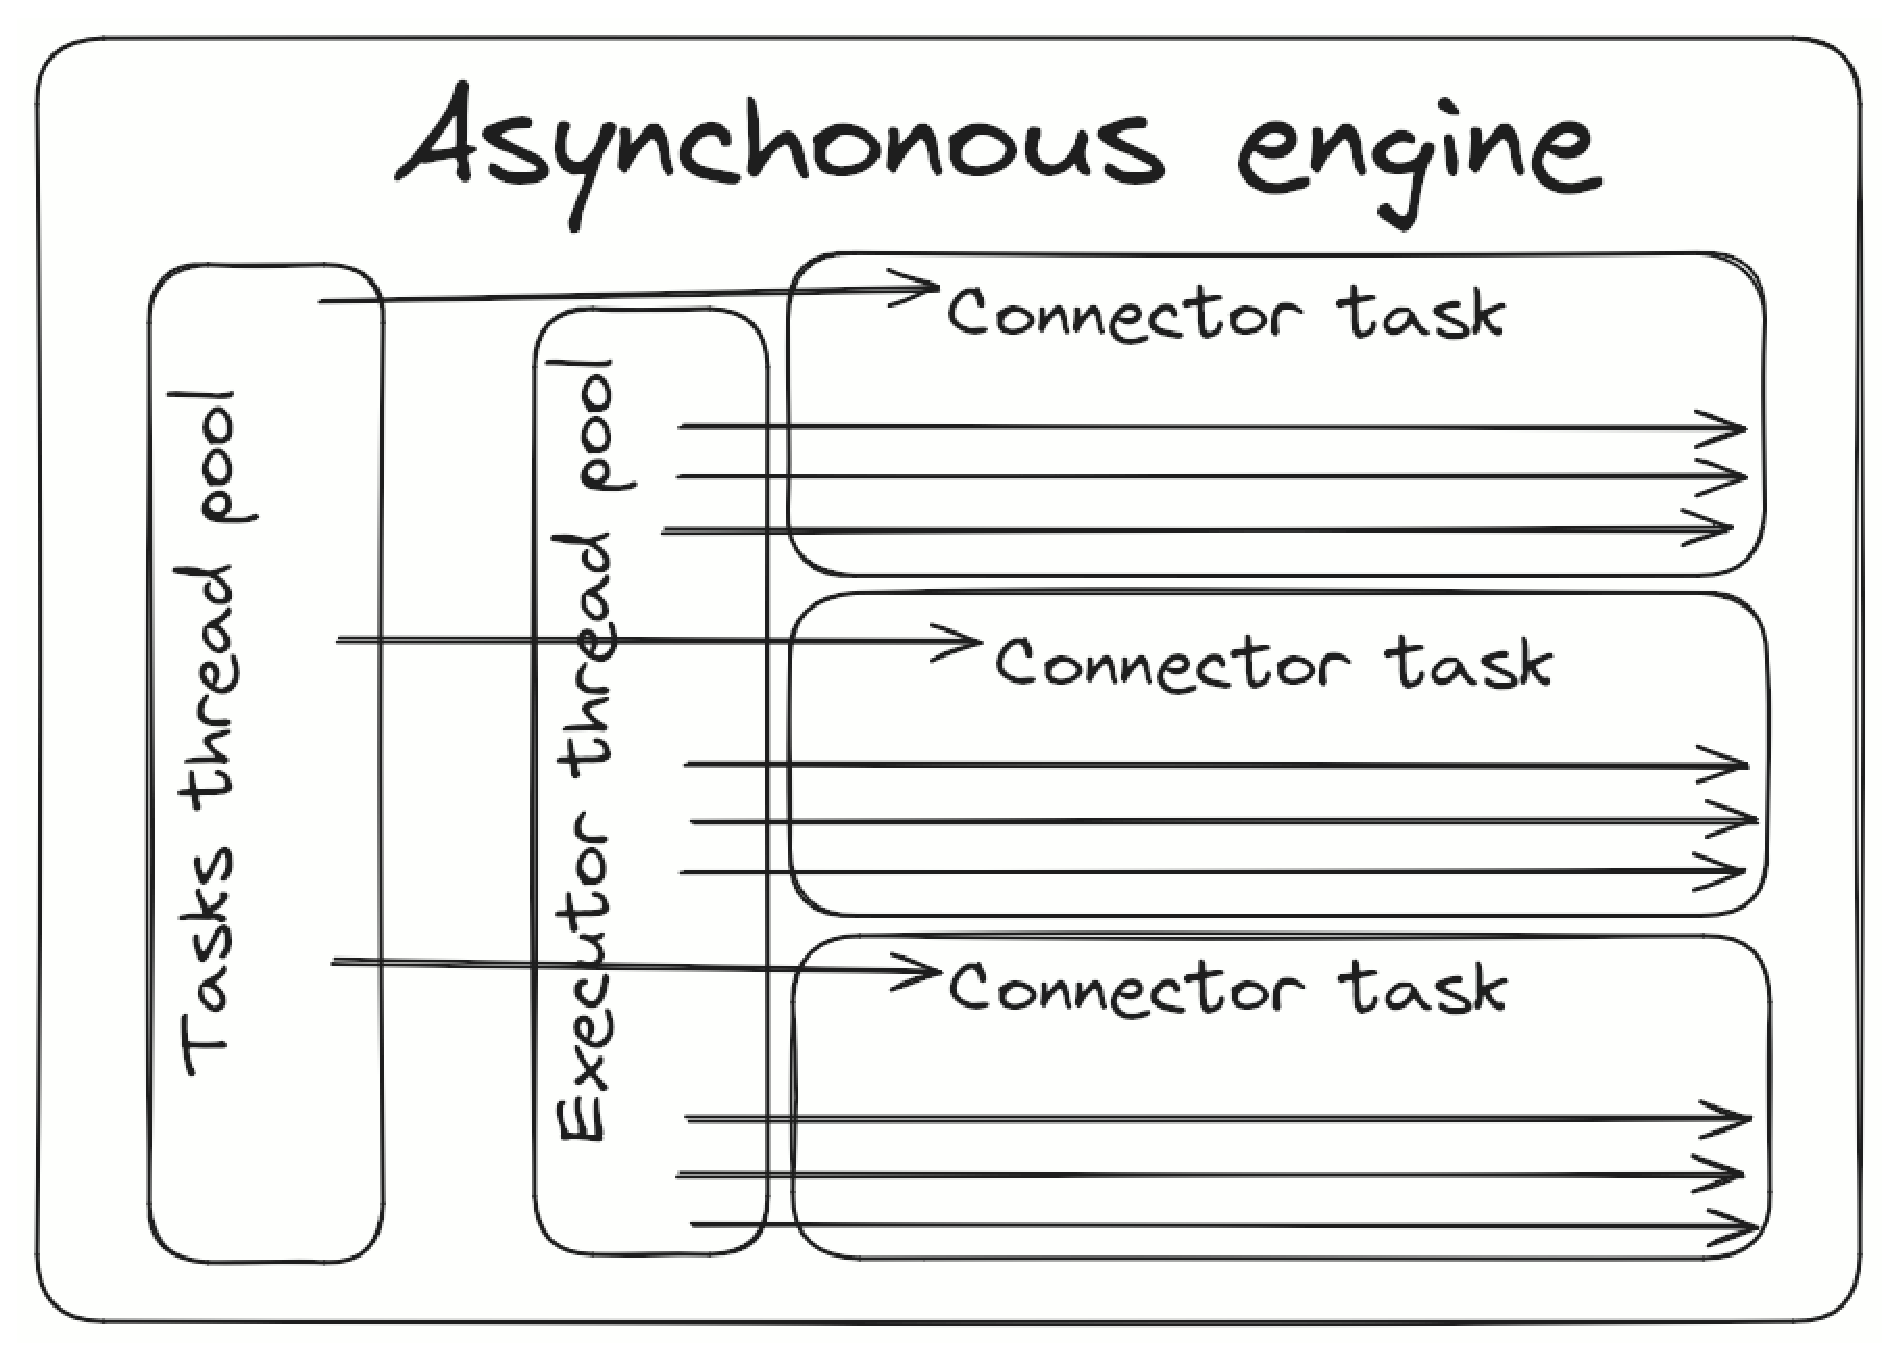
\includegraphics[height=6cm]{./img/async_engine.eps}
    \end{figure}
\end{frame}

\begin{frame}
    \frametitle{Resource}
    \begin{itemize}
        \color{blue}
        \item \href{https://github.com/debezium/debezium-design-documents/blob/main/DDD-7.md}{DDD-7: Asynchronous Debezium Embedded Engine}
        \item \href{https://github.com/debezium/debezium-design-documents/pull/8}{Discussion under DDD-7 PR}
        \color{black}
    \end{itemize}
\end{frame}


%%%%%%%%%%%%%%%%%%%%%%%%%%%%%%%%%%%%%%%%%%%%%%%%%%%%%%%%%%%%%%%%%%%%%%%%%%%%%%%%%%%%%%%%%%%%%%%%%
%%% BACKUP
%%%%%%%%%%%%%%%%%%%%%%%%%%%%%%%%%%%%%%%%%%%%%%%%%%%%%%%%%%%%%%%%%%%%%%%%%%%%%%%%%%%%%%%%%%%%%%%%%

% \begin{frame}
%     \centering
%     \huge{\textbf{Backup slides}}
% \end{frame}

\end{document}
